\begin{savequote}[75mm]
Some Quote.
\qauthor{Quoteauthor Lastname}
\end{savequote}

%For an example of a full page figure, see Fig.~\ref{fig:myFullPageFigure}.
\chapter{Model-Based Point Cloud Tracking}
\label{Chap:ModelBasedTracking}
\lettrine[lines=3, loversize=0.3]{\textcolor{DarkBlue}N}{ow that we have established} a reduced, stable world model in which voxels persist through occlusions, the next step is to adapt the general framework of Sequential Bayesian Estimation to track models within this 3D voxel model. The core concepts remain the same as discussed in Chapter \ref{Chap:VideoSegRelaxation}(for a brief introduction, see Appendix \ref{chap:SeqBayesEst}), and we will again use a bank of parallel particle filters, due to their robustness to noise (of which there is quite a bit in Kinect data) and ability to handle non-linear dynamics.

\section{Particle Filters in 3D}
The general concept of particle filtering remains the same as the 2D version discussed in Chapter \ref{Chap:VideoSegRelaxation}, with the primary changes lying in how we score individual particle predictions using the measurement model. The models have also been changed from 2D masks to 3D Point Cloud models which rely on point to point correspondence rather than a global histogram distance score. The dynamic model is an extension from 2D pixel position to real-world 3D coordinates which also include orientation. 

\section{Model Representation}
One of the main limitations of the 2D projected mask model discussed in Chapter \ref{Chap:VideoSegRelaxation} is that the masks of objects are not invariant to pose changes - in general, rotation of an object will change the shape of its mask and distribution of its color histogram. As we now have the ability to observe the full 3D shape of an object, we choose to represent objects as clusters of points which correspond to the exterior of the object. A visual representation of what such a model looks like is given in Figure \ref{fig:Object_Model}.

\missingfigure{Pointcloud representation of an object model}

Points are stored in an object-centered reference frame, and each contain an XYZ position, an RGB color for the point, as well as a surface normal vector. That is, each point $p$ of the model $k$ consists of a nine-dimensional vector: 

\begin{equation} \label{eqn:point}
p_k = [x,y,z,R,G,B,n_x,n_y,n_z],
\end{equation}
 
 and a model for an object $O_k$ consists of a vector of $n_k$ such points $p$:
 
 \begin{equation} \label{eqn:model}
 O_k = [p_0 ... p_{n_k}].
\end{equation}

It is important to note that the points of an object model given obove are model-relative - they must be transformed into the world coordinates in order to evaluate their fit to observations. This will be discussed further in the next Section.

\section{Dynamic Model}
\label{sec:Dynamic_model}
In the 2D tracker presented previously, the time-dependent state vector of a particle consisted of a position shift vector $\mathbf{p}_t=[p_x,p_y]$ and a velocity vector $\mathbf{v}_t=[v_x,v_y]$. The natural extension of this to 3D is to simply add a third $p_z$ and $v_z$ element to each. Of course we should note that the $x$ and$y$ dimensions here in our 3D representation are distinct from those in 2D, which represented pixel coordinates in the image plane. Here our positional coordinates represent real-world distances from a fixed origin (typically the camera ``pin-hole'' position).

While this straightforward extension gives us a reasonable 3D equivalent to our 2D tracked masks, we now have full 3D models, and so it makes sense to use a state vector which takes advantage of it. As such, we further extend the state vector for position and velocity to allow for rotations of the model around the object reference frame x-axis (roll - $\gamma$), y-axis (pitch - $\beta$), and z-axis (yaw - $\alpha$). This yields a position state vector for object $k$ at time $t$ of 
\begin{equation} 
 \mathbf{x}^k_t = [x, y, z, \gamma, \beta, \alpha],
\end{equation}
 and velocity state vector 
\begin{equation} 
 \mathbf{v}^k_t = [v_x, v_y, v_z, v_{\gamma}, v_{\beta}, v_{\alpha}].
\end{equation}
 
As before, motion is modeled using a constant velocity model in discrete time with uniform sampling period $\mathit{T}$, giving the dynamic model
\begin{equation} \mathbf{x}_t = \mathbf{x}_{t-1} + \mathbf{A}\mathbf{v}_{t-1} , \end{equation}
where
\todo[inline]{update this matrix to give 3d transform}
\begin{equation} \mathbf{A} = 
\begin{bmatrix}
 1 & \mathit{T} & 0  & 0 \\ 
 0 & 1 & 0 & 0\\ 
 0 & 0 & 1 & \mathit{T}\\ 
 0 & 0 & 0 & 1
\end{bmatrix} \end{equation}
and noise $\mathbf{v}_t$ is assumed to be zero mean Gaussian with fixed covariance.

\section{Measurement Model}

As points for the model are given in a model-centered frame of reference, we must transform model points to the world frame in order to evaluate them using a standard 3D affine transformation matrix:

\begin{equation} \mathbf{B} = 
\begin{bmatrix}
 \cos{\alpha}\cos{\beta} & \cos{\alpha}\sin{\beta}\sin{\gamma} - \sin{\alpha}\cos{\gamma} & \cos{\alpha}\sin{\beta}\cos{\gamma} + \sin{\alpha}\sin{\gamma}  & d_x \\ 
\sin{\alpha}\cos{\beta} & \sin{\alpha}\sin{\beta}\sin{\gamma} + \cos{\alpha}\cos{\gamma} & \sin{\alpha}\sin{\beta}\cos{\gamma} - \cos{\alpha}\sin{\gamma}  & d_y \\ 
 -\sin{\beta} & \cos{\beta}\sin{\gamma} & \cos{\beta}\cos{\gamma} & d_z \\ 
 0 & 0 & 0 & 1
\end{bmatrix} \end{equation}


\section{KL-Divergence Adaptation}
\section{Stratified Correspondence Sampling}
\todo[inline]{Provide simple experiment showing quality of track (maybe on VR Data) vs number of samples and particles.}
\todo[inline]{Also show result with occlusion? With some pure random samples added in?}
\section{Results on Virtual-Reality Data}
\begin{figure*}[!ht]
  \centering
  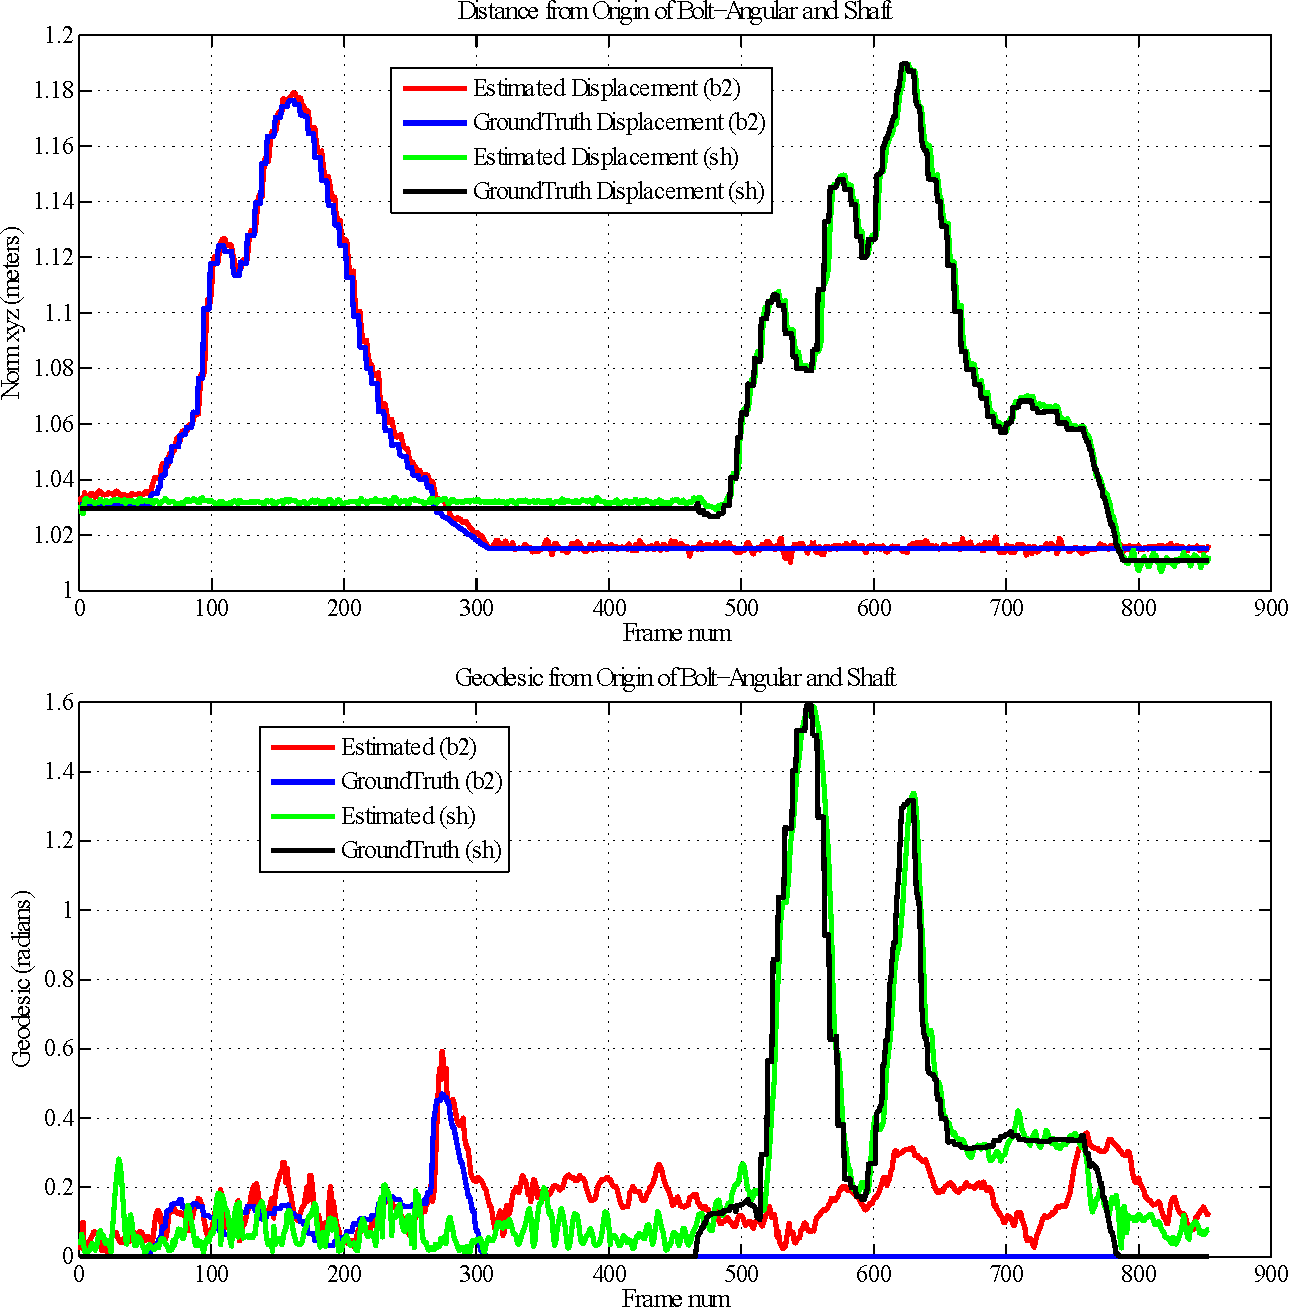
\includegraphics[width=\linewidth]{figures/Tracking/CombinedNoNoise.pdf}
  \caption[Tracked Output vs Ground Truth Artificial Sequence]{Tracked Output vs Ground Truth Artificial Sequence. The top panel shows position in terms of XYZ displacement and the bottom shows rotation in terms of geodesic. The location is generally tracked quite well, while the rotation is noisy due to the rotational symmetry of the two tracked objects (a bolt-angular and shaft).}
  \label{fig:CombinedNoNoise}
\end{figure*}

\begin{figure*}[!ht]
  \centering
  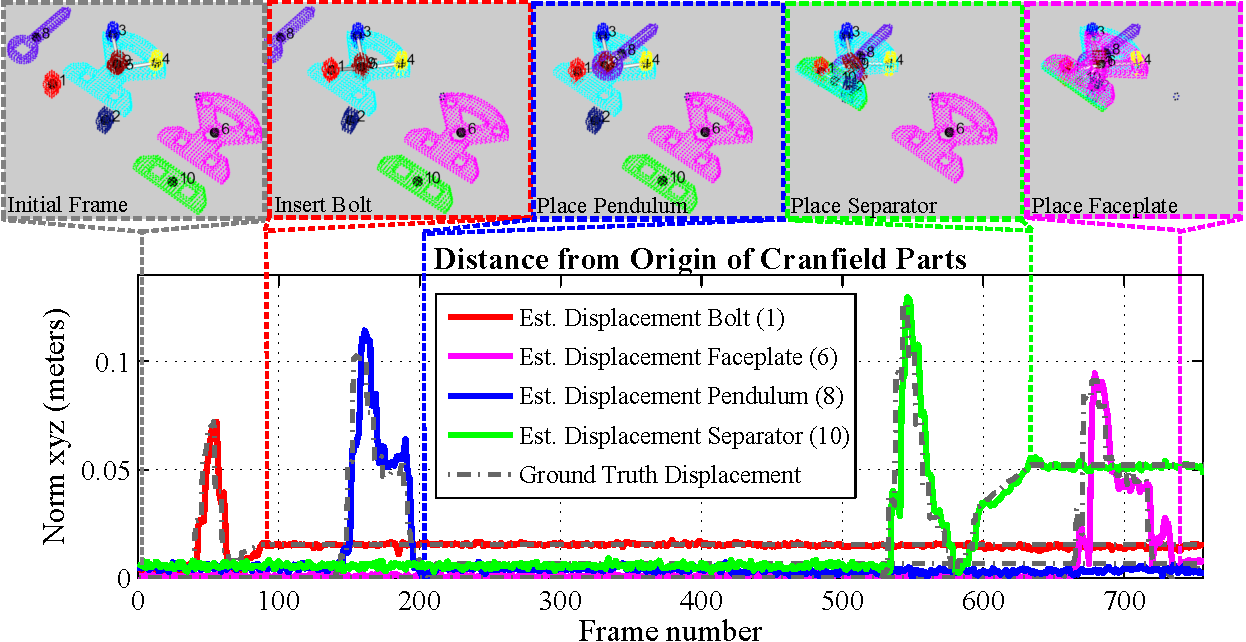
\includegraphics[width=\linewidth]{figures/Tracking/Action_Segmentation.pdf}
  \caption[Segmentation of Actions]{Segmentation of Cranfield Sequence into Keyframes - Tracked objects are monitored for when interactions between them occur, yielding keyframes which correspond to semantically important frames. Results here are shown for an artificial sequence with depth and RGB noise added.}
  \label{fig:ActionSegmentation}
\end{figure*}

\section{Results on Real Data}



